\section{Extending to multi-GPU}

\begin{frame}
	\frametitle{Towards exascale: multi-GPU systems}
	\begin{columns}
		\column{0.5\textwidth}
		\begin{itemize}
			\item Single GPU: powerful, but limited
			\item Distributed parallelism allows for scalable simulations
			\item Exascale-oriented machines are all hybrid systems
		\end{itemize}
		\begin{figure}
			\centering
			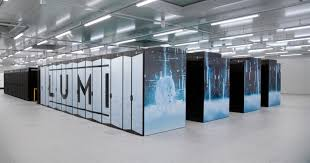
\includegraphics[width=0.8\textwidth]{images/LUMI.jpg}
		\end{figure}
		\column{0.5\textwidth}
		\begin{figure}
			\centering
			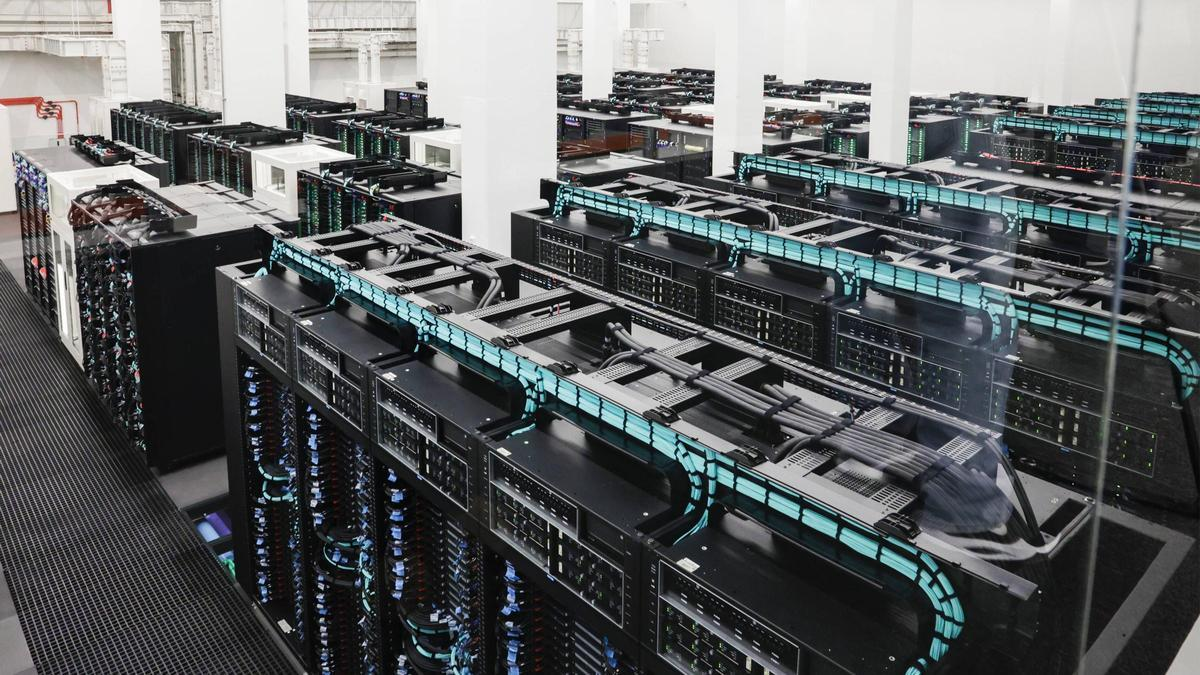
\includegraphics[width=0.8\textwidth]{images/MN5.jpg}
			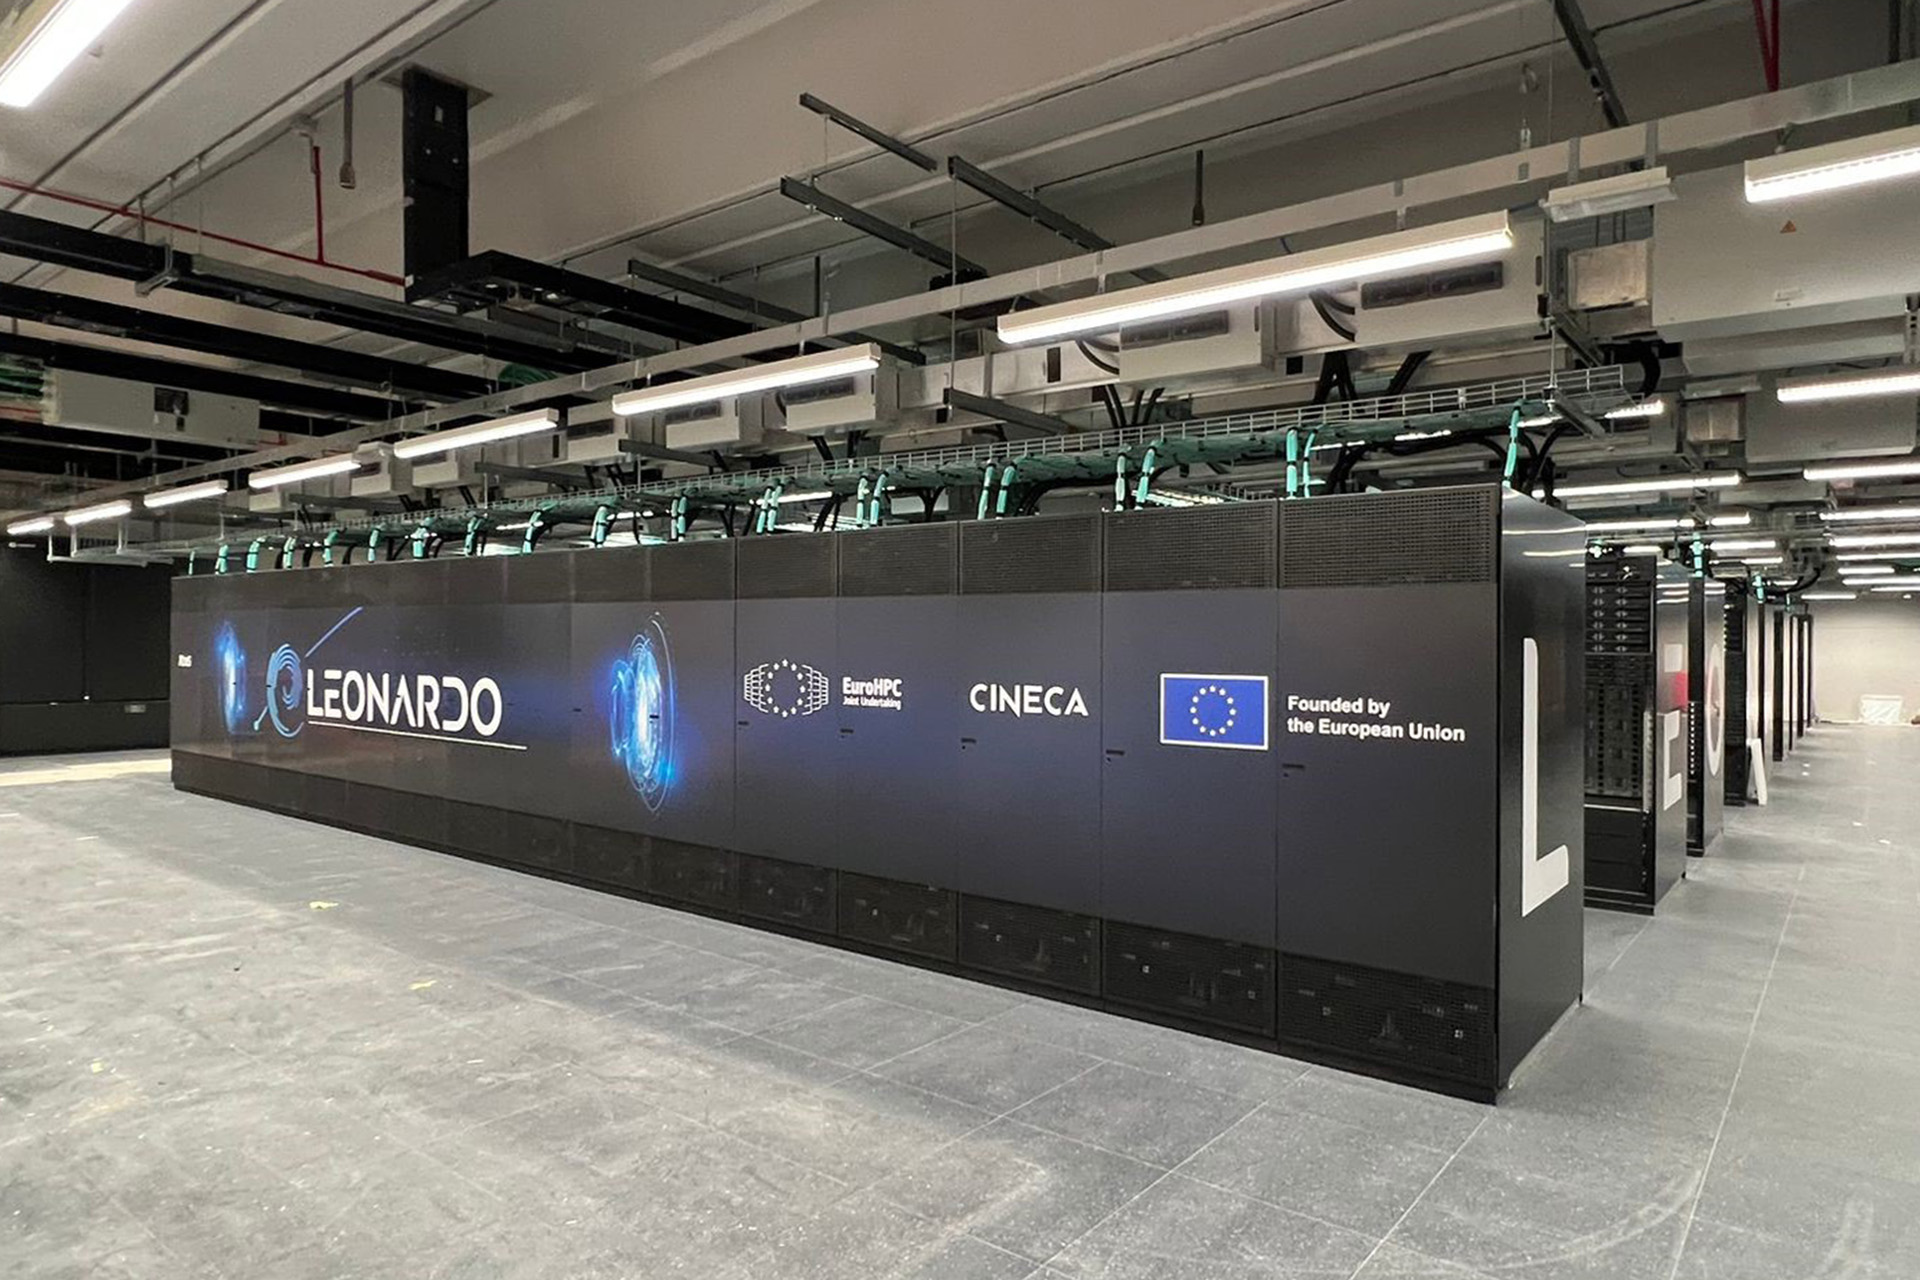
\includegraphics[width=0.8\textwidth]{images/leonardo.jpg}
		\end{figure}
	\end{columns}
\end{frame}

\begin{frame}
	\frametitle{Coarse-grained parallelism}
	\begin{columns}
		\column{0.5\textwidth}
		\begin{itemize}
			\item Domain decomposition: each "rank" computes part of the domain
			\item Partial computations require data exchange at interfaces
			\item Original mesh must be properly partitioned
			\item Strong scaling: fixed problem size, increase number of ranks (faster solution)
			\item Weak scaling: increase problem size with number of ranks (parallel efficiency)
		\end{itemize}
		\column{0.5\textwidth}
		\begin{figure}
			\centering
			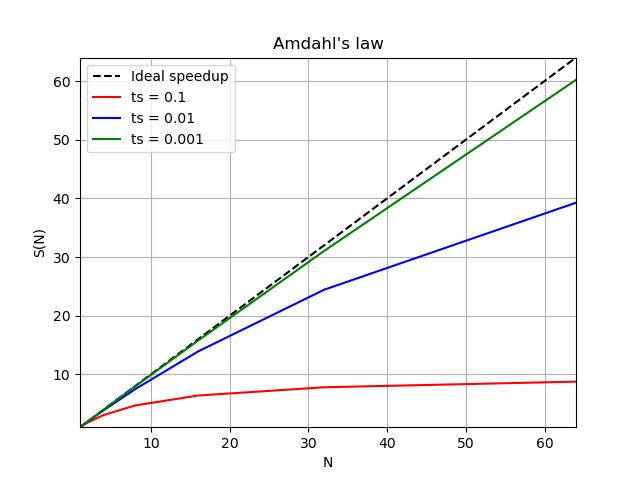
\includegraphics[width=0.74\textwidth]{images/amdahl.png}
			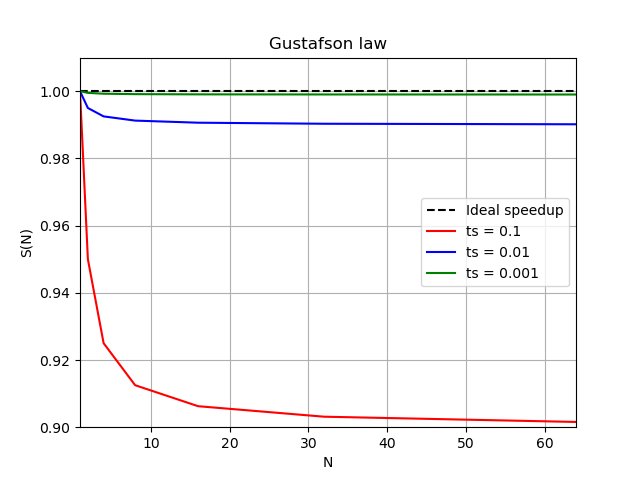
\includegraphics[width=0.74\textwidth]{images/gustafson.png}
		\end{figure}
		\end{columns}
\end{frame}

\begin{frame}
	\frametitle{Mesh partitioning}
	\begin{columns}
		\column{0.4\textwidth}
		\begin{itemize}
			\item Goal: Generate submeshes for all ranks
			\item Ideal case: perfect load balancing with minimal interface
			\item SOD2D uses the GeMPa library (\cite{bib:gempa})
			\item GeMPa: parallel partitioner based on Space-Filling Curves (SFC) method (\cite{bib:ric})
			\item Developed at BSC-CASE
		\end{itemize}
		\column{0.6\textwidth}
		\begin{figure}
			\centering
			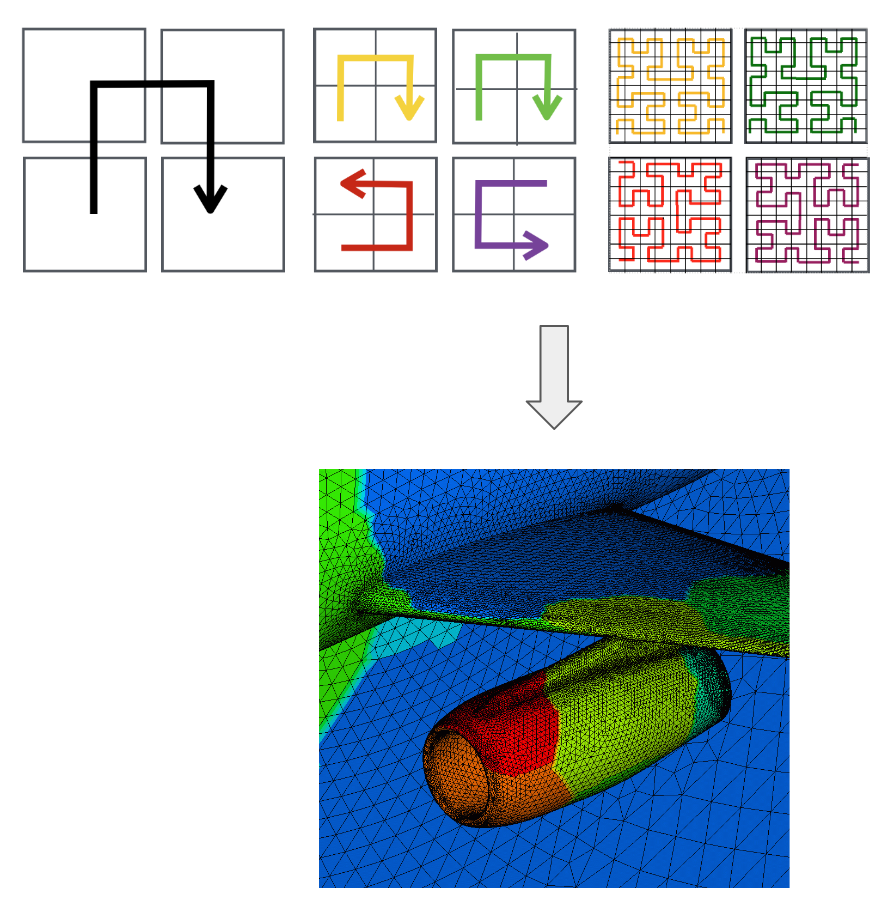
\includegraphics[width=0.95\textwidth]{images/gempa.png}
		\end{figure}
	\end{columns}
\end{frame}

\begin{frame}
	\frametitle{Communication strategy}
	\begin{columns}
		\column{0.5\textwidth}
		\begin{itemize}
			\item SOD2D requires exchanges to complete computed residuals from each subdomain
			\item Global-local numbering correspondence used to identify interfaces
			\item Computed arrays simply add missing info to communicating nodes
			\item Issue: many libraries and strategies available (MPI-2, MPI-3, OpenSHMEM...)
			\item Current choice: non-blocking CUDA-aware MPI Send-Recv messaging (iSR(C))
		\end{itemize}
		\column{0.5\textwidth}
		\begin{figure}
			\centering
			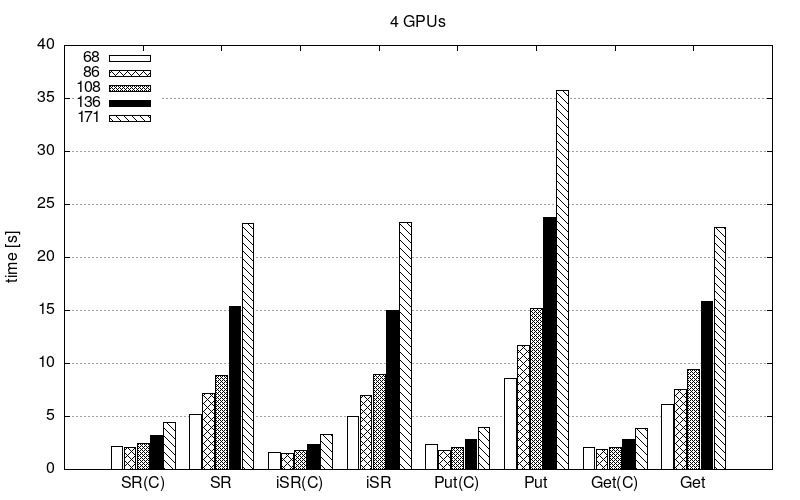
\includegraphics[width=0.95\textwidth]{images/mpiCompar/4gpuAll.png}
			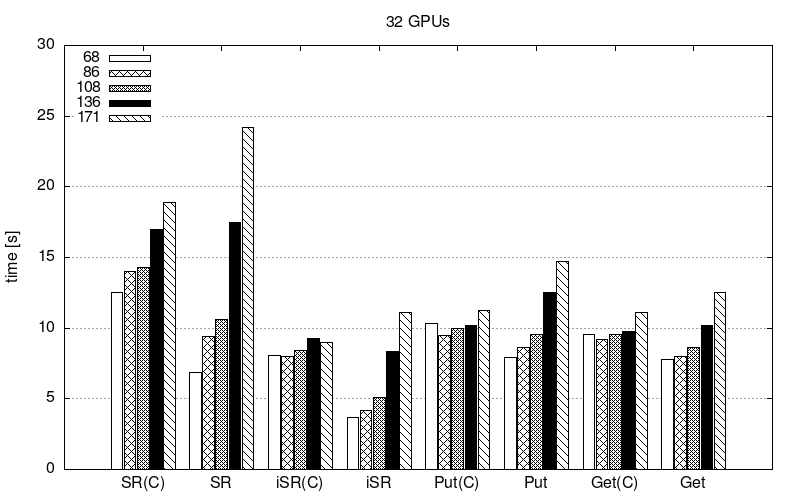
\includegraphics[width=0.95\textwidth]{images/mpiCompar/32gpuAll.png}
		\end{figure}
	\end{columns}
\end{frame}

\begin{frame}
	\frametitle{SOD2D scalability analysis}
	\begin{columns}
		\column{0.5\textwidth}
		\begin{itemize}
			\item Performed for both explicit and IMEX solvers
			\item Focus on finding optimal loading points for each system tested
			\item Test case: compressible TGV (multiple meshes)
			\item Meshes composed of 4th order HEXA-125 elements
		\end{itemize}

		\begin{block}{CTE-POWER}
			\begin{itemize}
				\item CPU: 2x IBM POWER9 8335-GTH 20C/40T @ 2.4Hz
				\item GPU: 4x NVIDIA V100 SXM2 16GB
				\item Single port Mellanox EDR interconnect
				\item Limited DtoD capabilities
			\end{itemize}
		\end{block}
		\column{0.5\textwidth}
		\begin{block}{ALCF Polaris}
			\begin{itemize}
				\item CPU: 1x AMD EPYC "Milan"
				\item GPU: 4x NVIDIA A100 SXM2 16GB
				\item HPE Slingshot 11 interconnect
			\end{itemize}
		\end{block}
		\begin{block}{MareNostrum5 ACC}
			\begin{itemize}
				\item CPU: 2x Intel Xeon Platinum 8460Y+ 40C @ 2.3GHz
				\item GPU: 4x NVIDIA Hopper H100 64GB HBM2
				\item 4x ConnectX-7 NDR200 InfiniBand
				\item Fully RDMA capable
			\end{itemize}
		\end{block}
	\end{columns}
\end{frame}

\begin{frame}
	\frametitle{Performance results (Explicit)}
	\begin{figure}
		\centering
		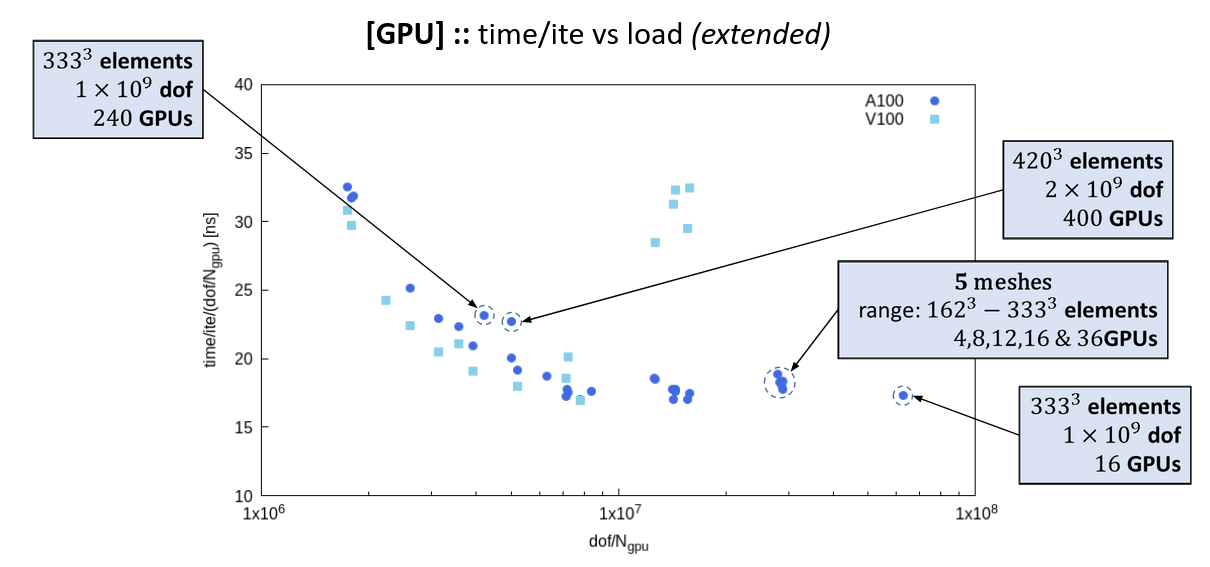
\includegraphics[width=0.95\textwidth]{images/uCurve.png}
		\caption{Scalability analysis of SOD2D explicit solver on CTE-POWER (V100) and Polaris (A100) clusters}
	\end{figure}
\end{frame}

\begin{frame}
	\frametitle{Performance results (IMEX)}
	\begin{figure}
		\centering
		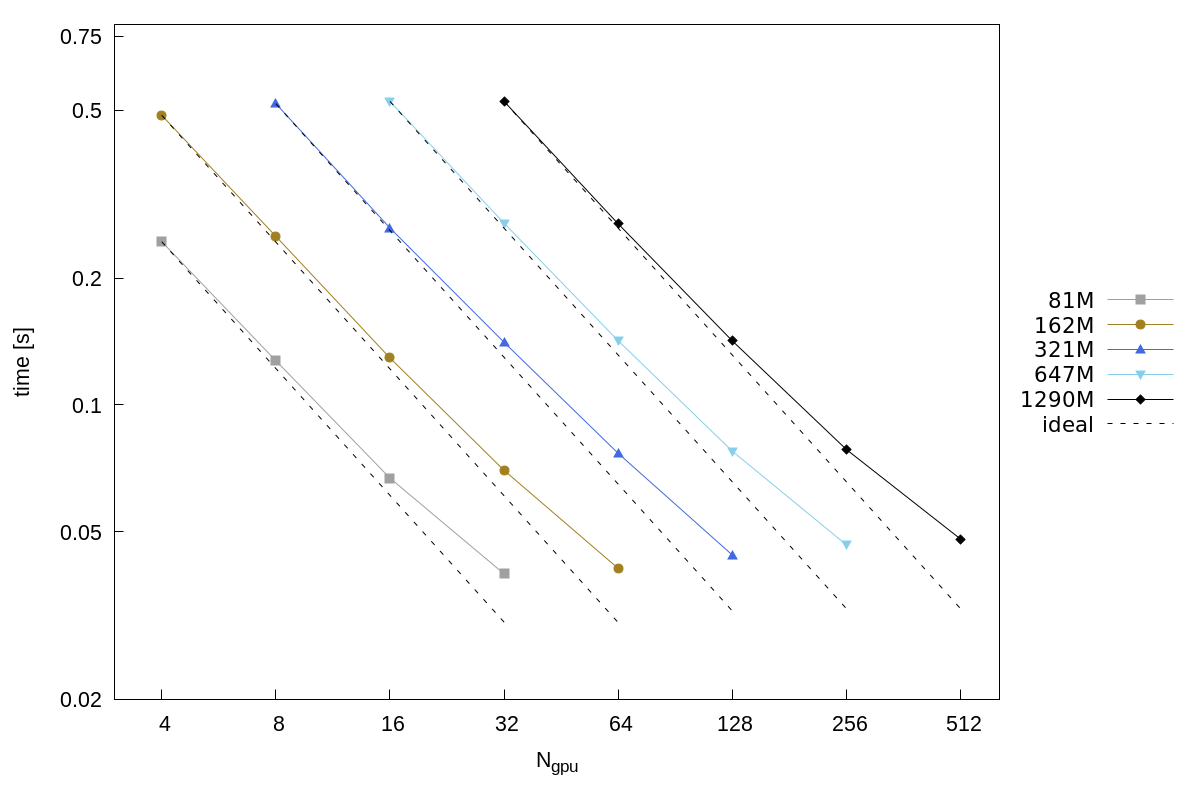
\includegraphics[width=0.8\textwidth]{images/comp_imex_MN5_H100_idealref_gpu.png}
		\caption{Scalability analysis of SOD2D IMEX solver on MN5 (H100) cluster}
	\end{figure}
\end{frame}